\chapter{Experiment 1 - Dataset and in-Network Transformation of MNIST}
\label{chap:five}

\section{Motivation}
In order to contextualize the results of the experiments conducted on malware data, we consider the methods presented there on the well-studied MNIST Database of Handwritten Digits~\cite{lecun1998mnist}.
MNIST is a benchmark in computer vision - since our baseline convolutional neural network is based on LeNet~\cite{lecun1998gradient}, we have a large body of research to compare to.
Additionally, MNIST serves as an introduction to the field of computer vision for many students and so our architectures and theories can be made more accessible in that context.
The current state of the art for MNIST~\cite{byerly2020branching}, achieved in January of this year achieves a 99.84\% accuracy.
The best results achieved in the original LeCun paper was 99.3\% accuracy and generally an accuracy greater than 97\% is considered to be good.

\section{Methodology}
In order to maintain consistency with our other findings, our methodology is nearly identical to experiments in Chapter~\ref{chap:three} and Chapter~\ref{chap:four}.
For our neural networks, we use stochastic gradient descent as our optimizer, with a learning rate of 0.001.
Results with other optimizers have been promising, and Adam~\cite{kingma2014adam} has been the optimizer of choice for many deep learning applications in the past few years. 
Model architectures are described below in detail.
We leverage the hardware described in Appendix~\ref{append:one} and perform two sub-experiments:
In our first sub-experiment, the network is trained for a maximum of 30 epochs and we use the early stopping technique to prevent overfitting.
Early stopping will end training early when some condition is met - in our case, we stop early if the network's loss has not decreased by 0.001 or more for two consecutive training epochs.
In our second sub-experiment, the network is trained for 1000 epochs without early stopping, and at each training epoch, the mutual information between the labels and the network, $I(Y; M)$ and the mutual information between the data and the network, $I(X; M)$ is computed.

\subsection{Mutual Information Computation}
Our mutual information graphs in figure~\ref{fig:mnist fc infoplane} and figure~\ref{fig:mnist conv infoplane} show the results of our mutual information computation.
As in previous literature~\cite{shwartz2017opening, saxe2019information}, during training, the gradients of each layer at the end of each epoch are recorded along with the L2 norm of the weights, the mean of the gradients, the variance of the gradients, and the activity in each layer.
After training, these gradients and kernel weights are used with the same training data and labels to estimate the mutual information via a Gaussian Mixture model~\cite{kolchinsky2017estimating}.
We use the recorded information and the datasets to compute pairwise distance estimators and for each layer, we compute the mutual information between the labels and the layer along with the mutual information between the data and the layer.
This estimate is:
$$-\sum_{i} p_i \ln \sum_{j} p_j \exp(-D(m_i || m_j))$$
where $p$ is the probability density of the dataset, X, and $m$ is the probability density estimate of our network layer, $M$.

\section{Models}\label{model_descriptions}
All code\footnote{Code is available at the following url: \url{https://github.com/erickgalinkin/jhu_masters}} was written in Python, using the Tensorflow 2, PyTorch, and Scikit-learn libraries.
Only the baseline models described in \ref{other models} used the Scikit-learn library, and only the Wavelet Convolutional network described in \ref{wavelet cnn} used PyTorch.
The remaining models all used the Tensorflow framework.

\subsection{Fully-Connected Neural Network}
The fully-connected neural network architecture accepts a flattened vector of length 768.
This vector is then fed to three densely connected layers, each with 256 ReLU-activated neurons.
The fourth and final output neuron is a single softmax layer, which provides a probability for each of the 10 MNIST classes.

\subsection{Standard Convolutional Neural Network}
Our convolutional neural network is a sequential model which accepts a 28 x 28 image as input.
This image is processed by an architecture comprised of a 5x5 convolution and a 3x3 convolution.
Each of these convolutional layers is followed by a max pooling layer.
The output of the second max pooling layer is flattened into 1-dimensional vector which is then processed by two densely connected layers of 128 neurons each. 
The final layer consists of a 10-neuron softmax layer, the same as our fully-connected network.

\subsection{Fourier Convolutional Neural Network}
Our Fourier ``Convolutional'' neural network is identical architecturally to our standard convolutional neural network, only with the convolutional layers replaced by Fourier layers.
Here, we put the word convolutional in quotes due to the fact that no actual convolution is performed.
To be more intellectually honest, we should refer to this network instead as a ``Fourier Transform Cross Product Network'', though this may confuse readers unfamiliar with the relationship.
In the interest of broad understanding, the term convolutional neural network is used when it helps clarify meaning even in spite of being a slight misnomer.

Specifically, the Fourier Convolutional Neural Network leverages a custom Fourier layer, which moves the data into Fourier space via the Fast Fourier Transform and then multiplies the transpose of the weight matrix with the input to the matrix.
Specifically, given an input $X^{(n)}$ and an output $A$, where the superscript is not an exponent, but instead indicates the layer of the input, the Fourier layer, $\ell$ acts on $X$:
\begin{align*}
X^{(n+1)} & = a \\
& = \ell^{(n)}(X^{(n)}) \\
& = \sigma(\mathcal{F}^{-1}(\mathcal{F}(X^{(n)})\cdot \mathbf{W}^{(n)\top}))
\end{align*}
Where $\mathcal{F}$ is the Fast Fourier Transform, $\sigma$ is the activation function - ReLU in this case - and $\mathbf{W}$ is the weight matrix for layer n.

\subsection{Wavelet Convolutional Neural Network} \label{wavelet cnn}
This input is then sent to the "wavelet layer" where it undergoes a Daubechies discrete wavelet transform.
This wavelet transform differs from the Morlet wavelet used in the modified dataset, since the continuous wavelet transform does not always invert nicely.
There are many potential wavelets that could be used~\cite{mallat1999wavelet} but since the discrete wavelet transform inverts cleanly and the Daubechies wavelet is easy to put into practice.53
The output is cast to a tensor which is multiplied against the transpose of the weight tensor.
This output then undergoes an inverse discrete wavelet transform with respect to the same mother wavelet.
As a result, the output of the layer remains the same shape as the input to the layer and so this architecture differs slightly from the other networks, since we do not use max pooling. 
The effect of this change to the architecture is not significant enough to be noteworthy.

The Wavelet Convolutional Neural Network implements similar functionality to our Fourier Neural Network, using the Continuous Wavelet Transform in lieu of the Fourier transform.
Due to the fact that there is a time component and a frequency component, the wavelet neural network has a different in-layer dimensionality than our other models, but is otherwise architecturally nearly identical.
These models were trained and evaluated on the same hardware as in \ref{chap:three}, with details in \ref{append:one}.
As before, the model accuracy was recorded over 100 trials and the average accuracy and average mean step time are reported.

\section{Results}
\begin{table}[h]
\centering	
\begin{tabular}{l|ll}
\textbf{Data and Architecture}  & \textbf{Test Accuracy} & \textbf{Mean Step Time} ($\mu$s) \\\cline{1-3}
Raw, Fully-Connected NN            & 97.73\%         & 29\\
Fourier, Fully-Connected NN        & 98.12\%         & 41\\
Wavelet, Fully-Connected NN        & 97.83\%         & 30\\
\hline
Raw, Convolutional NN              & 99.11\%         & 204\\ 
Fourier, Convolutional NN          & 99.10\%         & 237\\
Wavelet, Convolutional NN          & 99.10\%         & 212\\
\hline
Raw, Fourier NN                    & 98.45\%         & 959\\
Raw, Wavelet NN                    & 98.89\%         & 1068\\ 
\end{tabular}
\caption{Neural Network Results}
\label{Tab:test}
\end{table}

In this experiment, all of our models achieve accuracy over 97\% which is broadly considered to be the benchmark accuracy for ``passing'' MNIST. 
For all these combinations of architecture and transformation, the difference between our maximum accuracy score of 99.11\% and our minimum accuracy of 97.73\% is only 1.38\%.
Comparing the convolutional models in particular, the difference between the Raw, Fourier-transformed, and Wavelet-transformed data is only 0.01\%. 

\begin{figure}[h!]
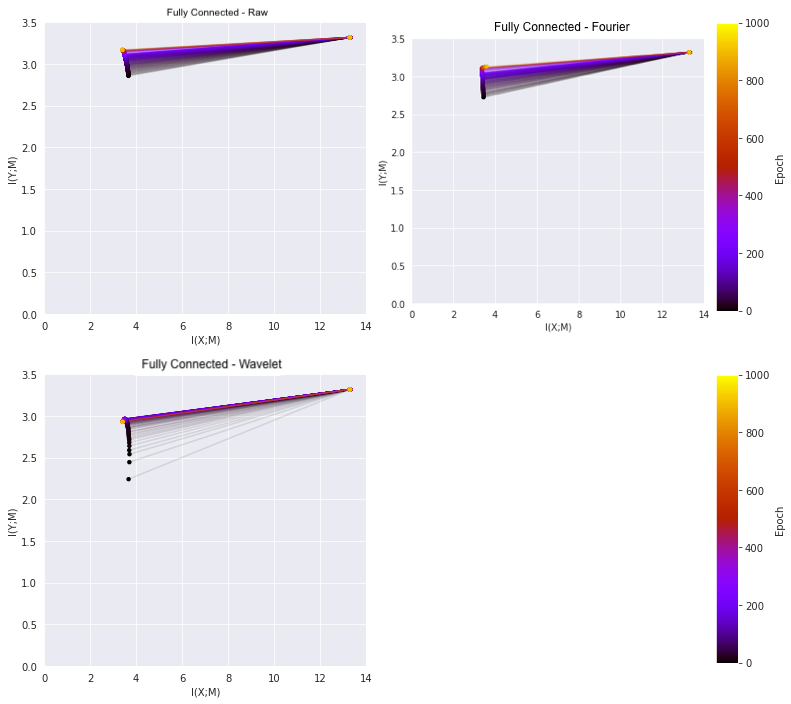
\includegraphics[width=0.75\textwidth]{mnist_fc_infoplane}
\caption{Fully-Connected Neural Network Information Plane. Reproduced using the upper bound methodology from Saxe~\cite{saxe2019information} for the first and last layer only over 1000 epochs.}
\label{fig:mnist fc infoplane}
\centering
\end{figure}
Over 1000 training epochs, the infoplane for the first and last layers of the neural net is quite similar for our fully-connected neural networks, quickly, and then more slowly increasing the information captured by the neural network about the labels. 
All three datasets are quite similar in terms of their information plane with respect to data and labels, with an upper bound for layer 3 which is within half a bit across all 3 datasets.

\begin{figure}[h!]
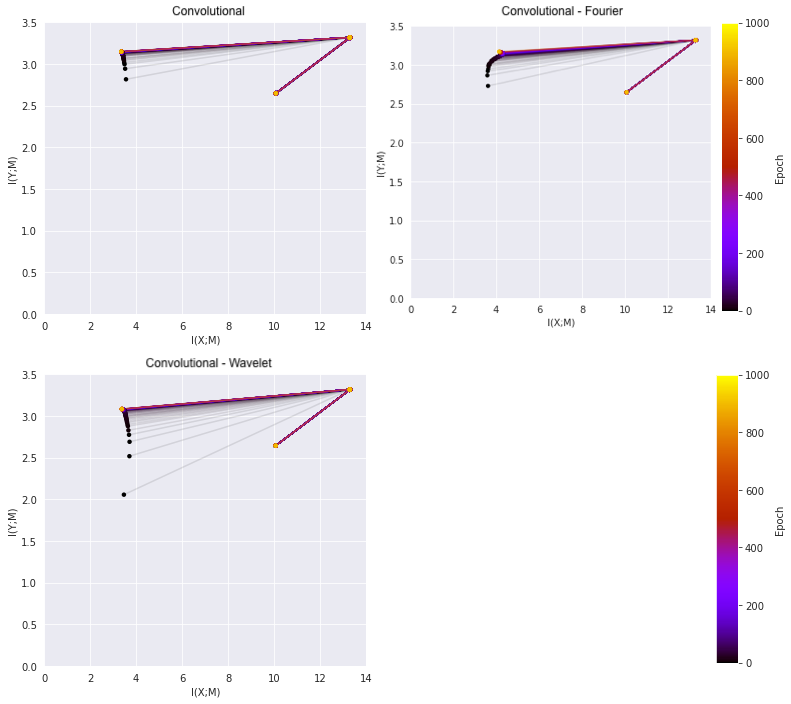
\includegraphics[width=0.75\textwidth]{mnist_conv_infoplane}
\caption{Convolutional Neural Network Information Plane}
\label{fig:mnist conv infoplane}
\centering
\end{figure}
We see quite similar results with the convolutional networks, though there is some odd behavior in layer 0 in late training epochs, where mutual information in layer 0 with respect to the dataset increases differently from our trend line. 
However, this phenomenon is consistent for our convolutional neural network across all 3 training data sets.
This consistency is surprising, and we discuss it in the context of our other experiments in chapter~\ref{chap:conclusion}.